\prefacesection{Appendix A: Presentation Slides}
% Creates a section titled "Appendix A: Presentation Slides" in the preface.
%
%
% Displaying the first two slides as an image.
\begin{figure}[h!]
    \centering
    % Centers the image on the page.
    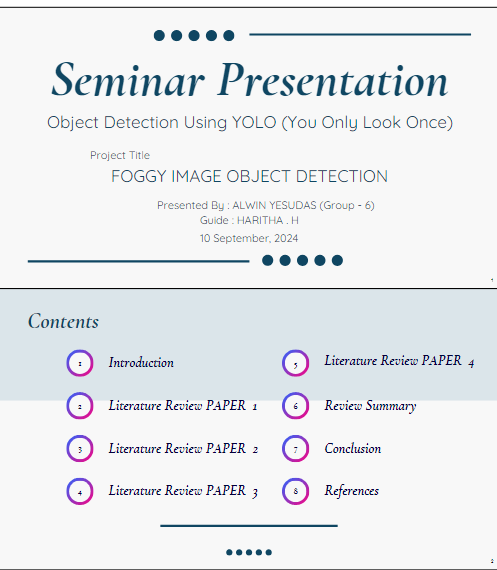
\includegraphics[width=1\textwidth]{images/Slide 1-2.png}
    % Includes an image file called "Slide 1-2.png" from the 'images' folder.
    % The image is scaled to the full width of the text area (\textwidth).
\end{figure}
% Ends the figure environment that contains the first two slides.
%
%
%
% Including slides 3 to 44 as a PDF with 2 slides per page.
\includepdf[nup=1x2, pages={3-44}, frame, pagecommand={\thispagestyle{plain}}]{pdfs/Seminar Presentation.pdf}
% \thispagestyle{plain}   ensures the page number is displayed
% Inserts pages 3 to 44 from a PDF file called "Seminar Presentation.pdf" located in the 'pdfs' folder.
% The option nup=1x2 places 2 slides per page in a 1-row, 2-column layout.
% The 'frame' option draws a border around each slide.
%
% End of the chapter
%
%